% !TeX TS-program = xelatex
\documentclass[10pt,a4paper]{article}
\usepackage[fontset=fandol, UTF8]{ctex}
\usepackage[margin=2cm]{geometry}
\usepackage[utf8]{inputenc}
\usepackage[T1]{fontenc}
\usepackage{listings}
\usepackage{enumitem}
\usepackage{color}
\usepackage{graphicx}
\usepackage{hyperref}
\usepackage{fourier}
\usepackage[scaled = 0.75]{beramono}
\usepackage{fancyhdr}
\usepackage{tikz}
\pagestyle{fancy}
\definecolor{myltgray}{rgb}{0.95,0.95,0.95}
\usepackage{textcomp}

\rhead{\raisebox{0.66ex}{\thepage}}
\lhead{\raisebox{0.66ex}{Julia 学习笔记}\ \ 
\includegraphics[width=0.409cm]{pen.png}}
\cfoot{}
\setlength\headheight{15pt}

\hypersetup{
    pdfstartview={FitH},
    pdftitle={Julia 学习笔记},
    pdfauthor={Yu Zhai},
    colorlinks=true,
    linkcolor=blue,
    urlcolor=blue
}

\lstdefinelanguage{commentonly}{ morecomment=[l]{\#} }
\lstset{
  basicstyle=\ttfamily,
  backgroundcolor=\color{myltgray},
  commentstyle=\emph,
  language=commentonly,
  upquote=true
 }

\setlength{\parskip}{2pt}%
%\setlength{\parindent}{0pt}

\begin{document}
\title{Julia 速览\footnote{英文版 commit: \texttt{d8cd0dd8a99d08c1a7499cb708ec3792751d24f4}。}}
\author{作者:Bogumi\l{} Kami\'n{}ski\\翻译:翟羽}
\date{2021年4月19日}
\maketitle

{\centering

\includegraphics[width=0.2\textwidth]{pen.png}\par
}

\tableofcontents

\section{引言}
本文旨在通过实例向程序员介绍 Julia 编程,
是 Julia 语言的简明概览。
\footnote{小火箭图标可由以下网址免费获取  \url{http://www.clipartlord.com/free-cartoon-rocketship-clip-art-2/}。
(译注:该站已殁。)}

执行这些例子的最简方法是将他们复制粘贴到 Julia 的输入-求值-打印循环(REPL) 里,或者粘贴到文件中然后使用 \lstinline|include| 功能运行。
两者不同之处在于前者每粘贴一条指令,终端中就会输出其结果。

若你的系统中缺少某包(package),则在 Julia REPL 中按下 \lstinline|]| 进入包管理器,
然后键入 \lstinline|add [包名]| 以安装该包。

这些年来的开发经验告诉我,管理多个 Julia 项目的最佳实践是分别使用不同的项目环境。
你可以阅读这篇博客
\url{https://bkamins.github.io/julialang/2020/05/18/project-workflow.html} 
了解更多。

本文仅具导论功能。以下重要主题本文未能涵盖,为 Julia 学习者所应知应会:
\begin{enumerate}[label=\arabic*),nolistsep]
  \item 参数类型(parametric types);
  \item 并行(parallel)与分布式处理(distributed processing);
  \item 进阶输入输出(I/O)操作;
  \item 进阶包管理;
  \item 与操作系统shell交互,参见 \lstinline|run|;
  \item 异常(exception)处理,参见 \lstinline|try|;
  \item 协程(coroutine)创建;
  \item 与 C、Fortran、Python 以及 R 交互。
\end{enumerate}
请参阅 Julia 最新版文档 \url{https://docs.julialang.org/} 
\footnote{译注:亦可参考完善中的中文文档 \url{https://docs.juliacn.com/latest/},但请以英文原文为准。} 以了解这些内容。

《 Julia 速览》 在以下 64 位版本的 Julia 下测试通过
(你可以在你的 Julia 会话中运行\lstinline|versioninfo()| 检查版本):
\begin{lstlisting}
Julia Version 1.4.2
Commit 44fa15b150* (2020-05-23 18:35 UTC)
Platform Info:
OS: Linux (x86_64-pc-linux-gnu)
CPU: Intel(R) Core(TM) i7-8550U CPU @ 1.80GHz
WORD_SIZE: 64
LIBM: libopenlibm
LLVM: libLLVM-8.0.1 (ORCJIT, skylake)
\end{lstlisting}

如你想使用 PDF 以外的格式阅读本文,其最简单的方法是克隆本项目
\sloppy\url{https://github.com/zhaiyusci/The-Julia-Express-zh-CN}\footnote{译注:原文地址为 \url{https://github.com/bkamins/The-Julia-Express}。}
至本地,
使用 pandoc 转换格式。
如执行
\begin{lstlisting}
pandoc -i julia_express.tex -f latex -t html5 -s -o julia_express.html
\end{lstlisting}
则输出 HTML 格式的文档。

欢迎一切建设性建议,可用电子邮件联系作者 \href{mailto:bkamins@sgh.waw.pl}{bkamins@sgh.waw.pl}。
\footnote{译注:如遇内容问题请联系作者,翻译问题请在 \href{https://github.com/zhaiyusci/The-Julia-Express-zh-CN/issues}{github issue} 中提出。}

\section{概览}

运行 \lstinline|julia| 可打开交互模式(REPL)。此模式下有用的命令有:
\begin{enumerate}[label=\arabic*),nolistsep]
  \item \lstinline|^D| (退出 Julia );
  \item \lstinline|^C| (中断计算);
  \item \lstinline|?| (进入帮助模式);
  \item \lstinline|;| (进入系统 shell 模式);
  \item \lstinline|]| (进入包管理模式);
  \item \lstinline|Ctrl-l| (清空屏幕);
  \item 表达式后接 \lstinline|;| 可阻止其值输出到 REPL中[脚本(script)模式不需要]。
\end{enumerate}

Julia REPL 基本功能举例如下(亦可在脚本中使用):
\begin{lstlisting}
  @edit max(1,2)      # 显示 max 函数当参数为 1, 2 时的定义
  varinfo()           # 列出全局变量及其类型
  cd("D:/")           # 将工作路径切换到 D:/ (在 Windows 下也可以用 / )
  pwd()               # 获取当前工作路径
  include("file.jl")  # 执行源文件
  exit(1)             # 退出 Julia,返回码(exit code)为 1 (默认为 0)
  clipboard([1,2])    # 将数据复制到系统剪贴板
  clipboard()         # 以字符串(string)格式加载系统剪贴板中的数据
\end{lstlisting}

你可以在系统 shell 里通过 \lstinline|julia script.jl| 运行 Julia 脚本。

将下列示例脚本保存至文件中并执行(在以后的章节中有更多例子):
\begin{lstlisting}
  """Eratosthenes 筛法函数文档( docstring )"""
  function es(n::Int) # 接受一个整数类型参数
      isprime = trues(n) # n 个元素的真(true)向量
      isprime[1] = false # 1 不是质数
      for i in 2:isqrt(n) # 在小于或等于 sqrt(n) 的整数中循环
          if isprime[i] # 条件求值
              for j in i^2:i:n # 步长为 i 的序列
                  isprime[j] = false
              end
          end
      end
      return filter(x -> isprime[x], 1:n) # 使用匿名函数筛选
  end
  
  println(es(100))         # 打印小于或等于 100 的全部素数
  @time length(es(10^6))   # 计算函数执行时间与内存使用
\end{lstlisting}

\section{基本字面值和类型}
下列者为基本标量字面值:
\begin{lstlisting}
  1::Int               # 64 位 Julia 中的 64 位(bit)整数,无溢出警告
  1.0::Float64         # 64 位浮点数,定义了 NaN, -Inf, Inf
  true::Bool           # 布尔型,可以是 true 或 false
  'c'::Char            # 字符,可以是 Unicode
  "s"::AbstractString  # 抽象字符串,可以有 Unicode,参见下述字符串(String) 
\end{lstlisting}
语法 \lstinline|x::Type| 指字面值(literal) \lstinline|x| 且断言(assert)其为 \lstinline|Type| 类型。
通常,类型断言并非必要,这里我们只是用它来指示每种字面值的类型。
所有的基本类型都是不可变的(immutable)。

以相同的方式可进行变量的类型断言,并可用于代码纠错。

Julia 中整数在 64 位 Julia 中是64位的,而在32位Julia 中是32位的。
这意味着 \lstinline|1::Int32| 断言在 64位Julia中会报错。
注意 \lstinline|Int| 是由 Julia 版本决定的常量,它要么是 \lstinline|Int64|,要么是 \lstinline|Int32|
(无符号整数 \lstinline|UInt|也类似)。

类型转换只能显式执行,没有自动类型转化。
这在函数调用中及其重要。
将 \lstinline|x| 转为 \lstinline|T| 类型的最简单方法是 \lstinline|T(x)|,如:
\begin{lstlisting}
  Int64('a')     # 字符到整数 (译注:结果为 97)
  Int64(2.0)     # 浮点数到整数
  Int64(1.3)     # 精度损失错误
  Int64("a")     # 没有可用的转化错误
  Float64(1)     # 整数到浮点数
  Bool(1)        # 转换为 true
  Bool(0)        # 转换为 false
  Bool(2)        # 转换错误
  Char(89)       # 整数到字符
  string(true)   # 将布尔型转为字符串(也可用于转换其他类型,注意首字母小写)
  string(1,true) # string 函数可以接收多个参数,并连接它们
  zero(10.0)     # 10.0对应类型的“零”
  one(Int64)     # Int64类型的“一”
\end{lstlisting}
广义的类型转换可由 \lstinline|convert(Type, x)|进行(一般当  \lstinline|x| 已经是 \lstinline|Type| 类型时, \lstinline|convert| 不再执行复制操作:
\begin{lstlisting}
  convert(Int64, 1.0) # 浮点数转为整数
\end{lstlisting}
Julia 无法准确进行类型转化时会抛出非精确转化错误。
\begin{lstlisting}
  convert(Int64, 1.3) # 将浮点数转换为整数 -> 抛出非精确转化错误
\end{lstlisting}
可使用 \lstinline|floor(Int64,1.3)|、 \lstinline|ceil(Int64,1.3)| 或 \lstinline|round(Int64,1.3)| 来解决这一问题。
字符串的解读可通过 \lstinline|parse(Type, str)| 完成:
\begin{lstlisting}
  parse(Int64, "1") # 以 Int64 类型解读字符串 "1"
\end{lstlisting}
多个参数自动提升为相同类型(若可行)可用 \lstinline|promote| 达成:
\begin{lstlisting}
  promote(true, BigInt(1)//3, 1.0) # BigFloat 类型元组(参见 Tuple) , true 转换为 1.0
  promote("a", 1)                  # 无法提升为相同类型
\end{lstlisting}
许多操作(算术、赋值)自动进行类型提升,故这是补足 Julia 没有类型自动转换规则的方法。

可通过如下方式查验值的类型:
\begin{lstlisting}
  typeof("abc")              # 返回 String, String是 AbstractString的子类型
  isa("abc", AbstractString) # true
  isa(1, Float64)            # false, 1 是整数而不是浮点数
  isa(1.0, Float64)          # true
  1.0 isa Number             # 另一种语法;true,Number (数)是一种抽象类型
  supertype(Int64)           # Int64 的父类型
  subtypes(Real)             # 抽象类型 Real 的子类型
\end{lstlisting}
我们也可以进行任意精度的算术运算及复数和分数的运算:
\begin{lstlisting}
  BigInt(10)^1000   # 大整数
  BigFloat(10)^1000 # 大浮点数,如需改变默认精度,可参考文档
  big(1.5)          # 对应大数类型的值,在此例是 BigFloat
  1 + 1im           # 复数
  123//456          # 使用 // 算符写分数
\end{lstlisting}

\begin{figure}
\centering
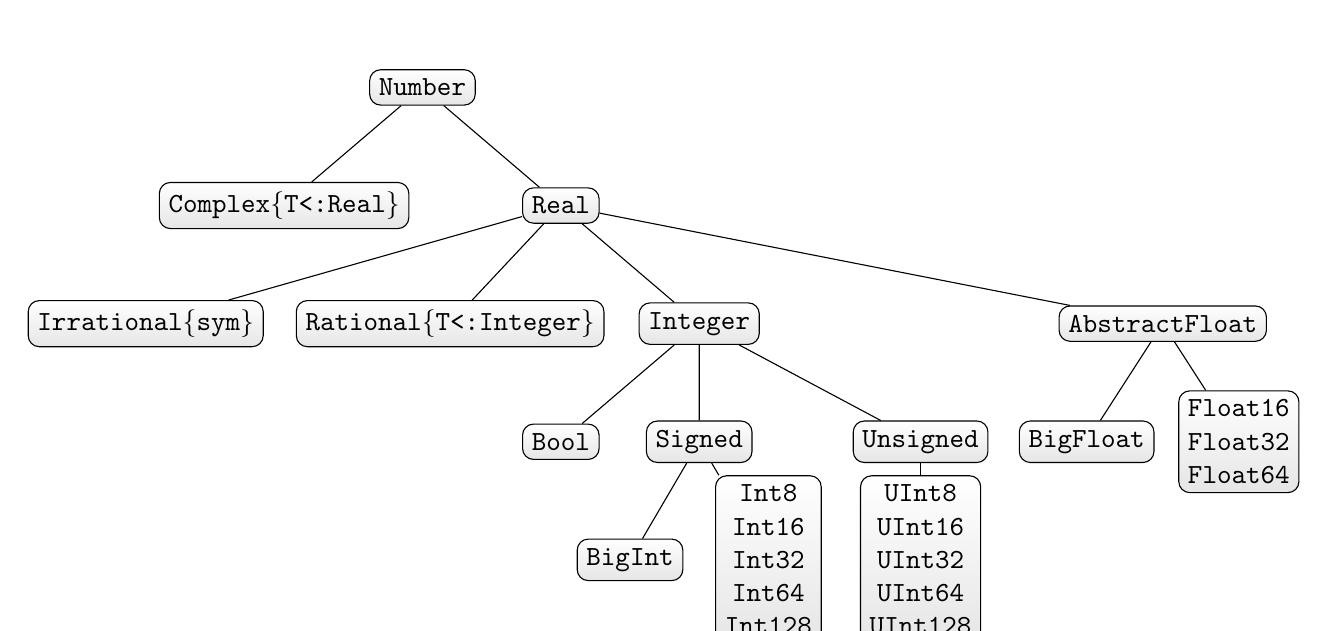
\begin{tikzpicture}[sibling distance=10em,
  every node/.style = {shape=rectangle, rounded corners,
    draw, align=center, font=\ttfamily,
    top color=white, bottom color=gray!20}]]
  \node {Number}
    child { node {Complex\{T<:Real\}} }
    child { node {Real}
        child { node {Irrational\{sym\}}}
        child[sibling distance=8em]{ node {Rational\{T<:Integer\}}}
        child { node {Integer}
            child[sibling distance=5em]{ node {Bool} }
            child[sibling distance=5em]{ node {Signed}
                child { node {BigInt} }
                child { node {Int8 \\ Int16 \\ Int32 \\ Int64 \\ Int128} }
            }
            child[sibling distance=8em]{ node {Unsigned}
                child { node {UInt8 \\ UInt16 \\ UInt32 \\ UInt64 \\ UInt128} }
            }
        }
        child[sibling distance=14.5em]{ node {AbstractFloat}
            child[sibling distance=5.5em]{ node {BigFloat} }
            child[sibling distance=5.5em]{ node {Float16 \\ Float32 \\ Float64} }
        }
    };
\end{tikzpicture}
\caption{数值类型的层级结构\label{fig:numeric}}
\end{figure}

全部标准数值类型的层级结构见图~\ref{fig:numeric}。

\section{特殊字面值与类型}
\begin{lstlisting}
  Any     # 所有对象皆为此类型
  Union{} # 所有类型的子类型,没有对象可以是该类型
  Nothing # 表示无的类型(值不存在),是 Any 的子类型
  nothing # Nothing 的唯一实例
  Missing # 表示遗失的类型(值存在但不知道),是 Any 的子类型
  missing # Missing 的唯一实例
\end{lstlisting}
此外 \verb|undef| 表示尚未完成初始化的对象元素(细节参见文档)。

\subsection{元组与命名元组}
元组(Tuple)是不可变的序列,其索引值(index)从 1 开始:
\begin{lstlisting}
  ()            # 空元组
  (1,)          # 一个元素的元组
  ("a", 1)      # 两个元素的元组
  ('a', false)::Tuple{Char, Bool} #元组类型断言
  x = (1, 2, 3)
  x[1]          # 1 (元素)
  x[1:2]        # (1, 2) (元组)
  x[4]          # 边界错误
  x[1] = 1      # 错误:元组是不可变的
  a, b = x      # 元组解包(unpacking), a==1, b==2
\end{lstlisting}
此外你可以给元组的元素取名[通过命名元组(NamedTuple)]:
\begin{lstlisting}
  NamedTuple()  # 一个空的命名元组
  (a=1,)        # 一个元素的命名元组
  (x="a", y=1)  # 两个元素的命名元组
  x = (p=1, q=2, r=3)
  x.p           # 访问元组的 p 元素
  typeof(x)     # NamedTuple{(:p, :q, :r),Tuple{Int64,Int64,Int64}},元素名是类型的一部分
\end{lstlisting}
命名元组可视为匿名 \lstinline|struct| ——参见下述复合类型(所以在测试子类型时它们和元组的行为不同,
这是本文不会涵盖的进阶主题,请参考 Julia 文档了解细节 \sloppy   \url{https://docs.julialang.org/en/latest/manual/types/} )。

\subsection{数组}
数组(Array)是可变的序列,且按引用传递。

可用以下函数创建数组:
\begin{lstlisting}
  Array{Char}(undef, 2, 3, 4) # 未初始化的 2x3x4 Char 类型数组
  Array{Int64}(undef, 0, 0)   # 退化的 0x0 Int64 类型数组
  zeros(5)             # Float64 类型的“零”构成的矢量
  ones(5)              # Float64 类型的“一”构成的矢量
  ones(Int64, 2, 1)    # Int64 类型的“一”构成的 2x1 数组
  trues(3), falses(3)  # 由 true 构成的矢量和 false 构成的矢量所构成的元组
  Matrix(I, 3, 3)      # 3x3 Bool 类型单位矩阵,需要先执行 using LinearAlgebra
  x = range(0, stop=1, length=11) # 有 11 个等间隔元素的迭代器(iterator)
  collect(x)           # 把迭代器转化为矢量
  1:10                 # 由 1 迭代至 10
  1:2:10               # 由 1 迭代至 9, 间隔为 2
  reshape(1:12, 3, 4)  # 3x4 类矩阵对象,逐列填充1到12
  fill("a", 2, 2)      # 2x2 数组,填充 "a"
  repeat(rand(2,2), 3, 2) # 2x2 随机矩阵,重复 3x2 次
  x = [1, 2]           # 两元素的矢量
  resize!(x, 5)        # 原位(in place)改变 x 的 尺寸,使之可以放 5 个值(用垃圾填充)
  [1]                  # 有一个元素的矢量(并非标量)
  [x * y for x in 1:2, y in 1:3] # 推导生成 2x3 矩阵
  Float64[x^2 for x in 1:4] # 将推导结果元素类型转换为 Float64
  [1 2]                # 1x2 矩阵(hcat 函数)
  [1 2]'               # 2x1 共轭矩阵(重复使用内存)
  permutedims([1 2])   # 2x1 矩阵(交换维度,新开内存)
  [1, 2]               # 矢量(连接) (concatenation)
  [1; 2]               # 矢量(vcat 函数)
  [1 2 3; 1 2 3]       # 2x3 矩阵(hvcat 函数)
  [1; 2] == [1 2]'     # false,数组维度不同
  hcat(1:2)==[1 2]'    # true,数组维度一致
  [(1, 2)]             # 一个元素的矢量
  collect((1, 2))      # 两个元素的矢量,通过解包元组得到
  [[1 2] 3]            # 按行连接(hcat)
  [[1; 2]; 3]          # 按列连接(vcat)
  tuple([1,2,3])       # 包含一个矢量的元组
  Tuple([1,2,3])       # 解包矢量构成的三个元素的元组
\end{lstlisting}
矢量(一维数组)是列矢量。

处理矩阵的大多数功能都在 \lstinline|LinearAlgebra| 包里。
此外,Julia 支持稀疏矩阵和分布矩阵(详见文档)。

常用数组函数有:
\begin{lstlisting}
  a = [x * y for x in 1:2, y in 1, z in 1:3] # 2x3 的 Int64 类型数组;长度为1的(singleton)维度被约化
  a = [x * y for x in 1:2, y in 1:1, z in 1:3] # 2x1x3 的 Int64 类型数组;长度为1的维度未被约化
  ndims(a)             # a 的维度
  eltype(a)            # a 中元素的类型
  length(a)            # a 中元素数目
  size(a)              # a 每一维度的大小所构成的元组
  axes(a)              # 数组索引范围(range)所构成的元组(译注:此处按文档重写)
  eachindex(a)         # 创建一个以最优方式访问 a 的可迭代对象(译注:此处按文档重写)
  CartesianIndices(a)  # 访问 a 的多维索引构成的数组(译注:此处按文档重写)
  LinearIndices(a)     # 访问 a 的一维索引构成的数组(译注:此处按文档重写)
  vec(a)               # 将一个数组转换为矢量(一维);复用内存
  dropdims(a, dims=2)  # 当 a 的第二维长度为1时,约去该维度
  sum(a, dims=3)       # 对第三维求和,相似地,该用法可以用于以下函数: mean, std,
                       # prod, minimum, maximum, any, all;
                       # 使用统计函数前需要 using Statistics
  count(>(0), a)       # 计算使条件成立的次数,类似地,可用于 all, any
                       # 注意这里我们用 >(0) 创建了一个匿名函数
\end{lstlisting}

访问函数:
\begin{lstlisting}
  a = 0:0.01:1         # 以 0.01 为间隔的区间
  a[1]                 # 标量 0.0
  a[begin]             # 标量 0.0 (第一个元素)
  a[end]               # 标量 1.0 (最后一个元素)
  a[begin:2:end]       # 区间中隔一个元素取一个
  view(a, 1:2:101)     # a 的 一个视角(view)(a 的一个子数组)(译注:对 view 的结果的操作会影响 a 本身)
  a[[1, 3, 6]]         # 将 a 视为 Array{Float64,1} 时的第1、3、6个元素
  lastindex(a)         # a 的最后一个 索引;firstindex 亦有类似用法 
\end{lstlisting}

长度为1的维度的处理:
\begin{lstlisting}
  a = reshape(1:12, 3, 4)
  a[:, 1:2]          # 3x2 矩阵
  a[:, 1]            # 3 个元素的矢量
  a[1, :]            # 4 个元素的矢量
  a[1:1, :]          # 1x4 矩阵
  a[:, :, 1, 1]      # 正确,3x4 矩阵
  a[:, :, :, [true]] # 正确,3x4x1x1 矩阵
  a[1, 1, [false]]   # 正确,0 个元素的 Array{Int64,1}
\end{lstlisting}

数组元素赋值:
\begin{lstlisting}
  x = collect(reshape(1:8, 2, 4))
  x[:,2:3] = [1 2]            # 错误;大小不一致
  x[:,2:3] .= [1 2]           # 正确,使用 . 广播
  x[:,2:3] = repeat([1 2], 2) # 正确
  x[:,2:3] .= 3               # 正确,需要使用 . 广播
\end{lstlisting}

数组是按引用(reference)赋值和传递的,故特别提供复制功能:
\begin{lstlisting}
  x = Array{Any}(undef, 2)
  x[1] = ones(2)
  x[2] = trues(3)
  a = x
  b = copy(x)     # 浅层复制
  c = deepcopy(x) # 深层复制
  x[1] = "Bang"
  x[2][1] = false
  a               # 与现在的 x 一模一样
  b               # 与原来的 x 相比,仅 x[2][1] 改变
  c               # 原来的 x 的内容
\end{lstlisting}

数组类型语法的例子:
\begin{lstlisting}
  [1 2]::Array{Int64, 2}      # Int64 类型的 2 维数组
  [true; false]::Vector{Bool} # Bool 类型的矢量
  [1 2; 3 4]::Matrix{Int64}   # Int64 类型的矩阵
\end{lstlisting}

数被视为 0 维容器:
\begin{lstlisting}
  x = 10   # 整数
  x[]      # 返回 10
  x[1,1]   # 也返回 10,末尾的 1被 Julia 忽略
  size(x)  # 空元组
  x = [10] # 一个元素的数组,可以用 [ ] 索引
  x[]      # 返回 10,这种用法仅在数组只有一个元素时可以奏效
\end{lstlisting}

\subsection{复合类型}
你可以定义、访问复合类型。以下是可变(mutable)复合类型的一个实例:
\begin{lstlisting}
  mutable struct Point
    x::Int64
    y::Float64
    meta
  end
  p = Point(0, 0.0, "Origin")
  p.x               # 访问域
  p.meta = 2        # 改变域的值
  p.x = 1.5         # 错误,数据类型不匹配
  p.z = 1           # 错误,没有这个域
  fieldnames(Point) # 获取所有的域名
\end{lstlisting}

类似地,你可以通过删除 \lstinline|mutable| 关键字来定义不可变复合类型(命名元组是匿名的不可变struct)。 

Julia 也支持联合(union)类型(详见 Julia 手册中 Type Unions 相关章节)。

最后你可以将你的类型定义为某抽象类型的子类型以将其适当的放在类型层级树中,你甚至可以定义自己的抽象类型(详见详见 Julia 手册中 Abstract Types 相关章节)。

\subsection{字典}
字典(Dict)是一种关联容器[键(key)-- 值(value)字典]:
\begin{lstlisting}
  x = Dict{Float64, Int64}()        # 将浮点数映射(map)为整数的空字典
  y = Dict("a"=>1, "b"=>2)          # 非空字典
  y["a"]                            # 访问元素
  y["c"]                            # 错误
  y["c"] = 3                        # 添加元素
  haskey(y, "b")                    # 检查 y 是否有 "b" 键
  keys(y), values(y)                # y 中的键和值
  delete!(y, "b")                   # 从字典中删除一个键,参见 pop!
  get(y,"c","default")              # 返回 y["c"],如果y["c"]不存在,返回 "default"
\end{lstlisting}
Julia 也支持集合(set),相似的用 \lstinline|Set| 可以构造集合(详见 Julia 文档)。

\section{字符串}
字符串(string)操作有:
\begin{lstlisting}
  "Hi " * "there!"       # 字符串连接
  "Ho " ^ 3              # 重复字符串
  string("a = ", 123.3)  # 使用打印方式构造
  repr(123.3)            # 返回show函数的输出
  occursin("CD", "ABCD") # 检查第一个字符串是否包含于第二个中
  "\"\n\t\$"             # C 语言风格的转义(escaping)字符串(注意 \$ 的转义)
  x = 123
  "$x + 3 = $(x+3)"      # 没有转义的 $ 用来原位求值(interpolation)
  "\$199"                # 要表示 $ 符号,你必须转义
  raw"D:\path"           # 原始(raw)字符串字面值,在表示 Windows 下的路径很有用
  s = "abc"              # 类型为 String 的字符串
  chop(s)                # 删除 s 的最后一个字符,返回一 SubString 类型对象
\end{lstlisting}

\lstinline|String| 和 \lstinline|SubString| 皆为 \lstinline|AbstractString| 的子类型。
\lstinline|SubString| 可避免复制字符串。
通常,当写自己的程序时,应假设用户会使用 \lstinline|AbstractString|。

与 Perl 兼容的(PCRE) 正则表达式处理:
\begin{lstlisting}
  r = r"A|B"           # 创建新的正则表达式
  occursin(r, "CD")    # false,不匹配
  m = match(r, "ACBD") # 找到第一处正则表达式匹配,详见 Julia 文档
\end{lstlisting}

还有很多字符串函数——详见 Julia 文档。

警告!你可以用索引字符串,例如 \lstinline|"abc"[1]| 会返回字符 \lstinline|'a'|。
然而,Julia 是用 UTF-8 来编码标准字符串的,而索引是按字节而不是字符,所以你需要理解UTF-8编码才能正确地索引。详见 Julia 文档。

\section{程序结构}
将值联系到变量上的最简单方法是赋值:
\begin{lstlisting}
  x = 1.0          # x 指向一个 Float64 的值
  x = 1            # 现在 x 指向了 Int32 或 Int64 的值(取决于机器)
\end{lstlisting}

表达式可以用 \lstinline|;| 或者 \lstinline|begin end| 块结合在一起:
\begin{lstlisting}
  x = (a = 1; 2 * a) # 此后  x = 2; a = 1
  y = begin
    b = 3
    3 * b
  end              # 此后 y = 9; b = 3
\end{lstlisting}

标准的程序结构有:
\begin{lstlisting}
  if false    # if 从句需要 Bool 测试
      z = 1
  elseif 1 == 2
      z = 2
  else
      a = 3
  end         # 此后 a = 3,z 未定义

  1==2 ? "A" : "B" # 标准三元操作符

  i = 1
  while true
      global i += 1
      if i > 10
        break
      end
  end

  for x in 1:10    # x 在区间中,这里可以用 = 代替 in
      if 3 < x < 6
          continue # 跳过一次迭代
      end
      println(x)
  end              # x 在此循环的内部作用域被定义
\end{lstlisting}

你可以定义自己的函数(function):
\begin{lstlisting}
  f(x, y = 10) = x + y           # 新函数 f 的单行定义,y 默认值是 10
                                 # 返回最后一个表达式的结果
  function f(x, y=10)            # 和上面一样,但允许多个表达式
      x + y                      # 在函数体内
  end
  f(3, 2)                        # 简单的调用,返回 5
  f(3)                           # 返回 13
  (x -> x^2)(3)                  # 匿名函数的调用
  () -> 0                        # 没有参数的匿名函数
  h(x...) = sum(x)/length(x) - mean(x) # 可变参数的函数;x 是元组; 需要 using Statistics
  h(1, 2, 3)                     # 结果为 0
  x = (2, 3)                     # 元组
  f(x)                           # 错误:我们企图把10加到 (2, 3) 上
  f(x...)                        # 正确,元组解包
  s(x; a = 1, b = 1) = x * a / b # 有关键词参数 a 和 b 的函数
  s(3, b = 2)                    # 带关键词参数的调用
  q(f::Function, x) = 2 * f(x)   # 函数可以当作参数传递;这里我们要求 f 是一个函数
  q(x -> 2x, 10)                 # 返回 40,不必在 2x 中间写乘号(代表 2*x)
  q(10) do x                     # 通过 do 结构创建匿名函数,例如在输入输出有用
    2 * x
  end
  m = reshape(1:12, 3, 4)
  map(x -> x ^ 2, m)             # 包含转换过数据的 3x4 数组
  filter(x -> bitstring(x)[end] == '0', 1:12)  # 在区间里筛选偶数的亮眼方法
  ==(1)                          # 返回一个检查是否等于1的函数
  findall(==(1), 1:10)           # 找到所有等于 1 的元素的索引,相似地:findfirst, findlast
\end{lstlisting}

习惯上以 \lstinline|!| 结尾地函数会原位修改其参数。参见本文档中的 \lstinline|resize!|。

默认函数参数自左向右求值:
\begin{lstlisting}
  y = 10
  f1(x=y) = x; f1()      # 10
  f2(x=y,y=1) = x; f2()  # 10
  f3(y=1,x=y) = x; f3()  # 1
  f4(;x=y) = x; f4()     # 10
  f5(;x=y,y=1) = x; f5() # 10
  f6(;y=1,x=y) = x; f6() # 1
\end{lstlisting}

Julia 中\textsf{函数}可以有多个\textsf{方法}(method)。
每个方法对应函数的一组参数类型。
这种行为叫多重派发(multiple dispatch)并且只对位置(positional)参数有效。
以下是一些简短的例子。详见 Julia 的 Methods 章节。
\begin{lstlisting}
  g(x, y) = println("all accepted") # g 函数接收任何类型 x 和 y 的方法
  function g(x::Int, y::Int)        # 当 x 和 y 均为 Int 型调用的方法
    y, x
  end
  g(x::Int, y::Bool) = x * y        # 当 x 为 Int,y 为 Bool 时的方法
  g(1.0, 1)                         # 第一个定义被调用
  g(1, 1)                           # 第二个定义被调用
  g(1, true)                        # 第三个定义被调用
  methods(g)                        # 列出 g 的所有方法
  t(; x::Int64 = 2) = x             # 单个关键词参数
  t()                               # 返回 2
  t(; x::Bool = true) = x           # 没有对关键词参数的多重派发,函数定义被覆盖
  t()                               # true;旧函数被覆盖
\end{lstlisting}

\section{变量作用域}
以下结构创建新的变量作用域(variable scope):
\lstinline|function|、\lstinline|while|、
\lstinline|for|、\lstinline|try/catch|、
\lstinline|let|、\lstinline|struct|、\lstinline|mutable struct|。

你可以将变量定义为:
\begin{itemize}
  \item \lstinline|global|:在当前模块的全局作用域使用变量;
  \item \lstinline|local|: 在当前作用域定义新变量;
  \item \lstinline|const|: 确保变量类型是常量(仅全局)。
\end{itemize}

特殊情况:
\begin{lstlisting}
  t                  # 错误,变量 t 不存在
  f() = global t = 1
  f()                # 调用后 t 在全局作用域被定义

  function f1(n)
    x = 0
    for i = 1:n
      x = i
    end
    x
  end
  f1(10)            # 10;在循环内我们使用了外部局域变量

  function f2(n)
    x = 0
    for i = 1:n
      local x
      x = i
    end
    x
  end
  f2(10)            # 0;在循环内我们使用了新的局域变量

  function f3(n)
    for i = 1:n
      h = i
    end
    h
  end
  f3(10)            # 错误;h 在外部作用域未定义

  const x = 2
  x = 3 # 警告,常量的值被改变;但你永远不应该这样写,这会导致编译好的代码失效
  x = 3.0 # 错误,类型错误

  function f()
      x::Int = 1
      x = 2.5 # 当调用 f() 时会报错,因为 x 必须是 Int
  end
\end{lstlisting}
全局常量会加速代码执行,因为编译器知道其类型。

循环和推导在每次迭代时都重新给变量赋值,故可以安全地在迭代中用他们创造闭包(closure):
\begin{lstlisting}
  Fs = Array{Any}(undef, 2)
  for i in 1:2
    Fs[i] = () -> i
  end
  Fs[1](), Fs[2]() # (1, 2)
\end{lstlisting}

\section{模块}
模块(module)将代码封装起来,每个模块有他们自己的全局命名空间(Julia REPL 的模块名是 \lstinline|Main|)。
\begin{lstlisting}
  module M # 模块名
  export x # 模块向外界所暴露的
  x = 1
  y = 2 # 隐藏变量
  end

  varinfo(M) # 列出导出的变量
  x       # 在全局作用域中找不到
  M.y     # 可以直接访问变量

  # 导入所有导出的变量
  # 也可以用此法加载标准包,但不需要 . 前缀
  using .M

  # 将 y 导入全局作用域 (即使其没有被导出)
  import .M.y
\end{lstlisting}
给其他模块中的变量绑定值是不可以的。如下是常常让人们惊讶的经典小例子:
\begin{lstlisting}
  sin(1) # 成功
  sin = 1 # 失败,在模块 Main 里你不能给模块 Base 里的变量绑定值
  cos = 1 # 成功,因为cos还没有被调用,故还没有从 Base 导入到 Main
  cos # 返回 1
  cos(1) # 失败,cos 在 Main 模块绑定了 1
  Base.cos(1) # 成功
\end{lstlisting}

\section{操作符}
Julia 使用标准的操作符,而有如下的小技巧:
\begin{lstlisting}
  true || false    # 二元或算符(仅单元素使用),|| 和 && 采短路求值
  [1 2] .& [2 1]   # 逐位(bitwise)与算符 [以 . 向量化(vectorize)]
  1 < 2 < 3        # 支持连锁条件(chaining conditions)(仅单元素使用,不可用 . 向量化)
  [1 2] .< [2 1]   # 向量化的操作符需要前缀 .
  x = [1 2 3]
  2x + 2(x .+ 1)   # 字面值和变量间的乘号及字面值或变量与左括号间的乘号可省略
  y = [1, 2, 3]
  x + y  # 错误:维度不匹配
  x .+ y # 3x3 矩阵,维度广播(broadcasting)
  x + y' # 1x3 矩阵
  x * y  # 数组乘法,单元素矢量(不是标量)
  x .* y # 逐元素(element-wise)乘法,3x3 数组

  x == [1 2 3]  # true,对象值一样
  x === [1 2 3] # false,对象并非同一

  z = reshape(1:9, 3, 3)
  z + x  # 错误:维度不匹配
  z .+ x # x 纵向广播
  z .+ y # y 横向广播

  # 长度为1的维度的显式广播
  # 对每一个数组元素,函数 + 都被调用
  broadcast(+, [1 2], [1; 2])
  # 使用 . 操作符广播
  using Random
  length([randstring(10) for i in 1:5]) # 5:数组的长度
  length.([randstring(10) for i in 1:5]) # 由 10 构成的 5个元素的数组:字符串的长度
\end{lstlisting}

函数广播的例子:
\begin{lstlisting}
  t(x::Float64, y::Float64 = 1.0) = x * y
  t(1.0, 2.0)               # 成功
  t([1.0 2.0])              # 错误
  t.([1.0 2.0])             # 成功
  t([1.0 2.0], 2.0)         # 错误
  t.([1.0 2.0], 2.0)        # 成功
  t.(2.0, [1.0 2.0])        # 成功
  t.([1.0 2.0], [1.0 2.0])  # 成功
  t.([1.0, 2.0], [1.0 2.0]) # 成功
\end{lstlisting}

\section{基本常用函数}
\begin{lstlisting}
  show(collect(1:100)) # 显示对象的字符串表示
  eps()             # 从 1.0 到下一个可表示的 Float64 类型数的差距(译注:机器相对误差)
  nextfloat(2.0)    # 下一个可表示的浮点数,类似地,提供了 prevfloat
  isequal(NaN, NaN) # true
  NaN == NaN        # false
  NaN === NaN       # true
  isequal(1, 1.0)   # true
  1 == 1.0          # true
  1 === 1.0         # false
  0.0 == -0.0       # true
  0.0 === -0.0      # false
  isfinite(Inf)     # false,类似地提供了 isinf, isnan
  fld(-5, 3), mod(-5, 3) # (-2, 1), 朝向负无穷的整数除法
  div(-5, 3), rem(-5, 3) # (-1, -2), 朝向零的整数除法
  findall(x -> mod(x, 2) == 0, 1:8) # 找到使函数为真的索引
  x = [1 2]; identity(x) === x # true,返回参数本身
  @info "Info"      # 打印信息,类似地有 @warn 和 @error (参见 Logging 模块)
  ntuple(x->2x, 3)  # 通过以值 1、2、3 调用 x->2x 创建元组
  @isdefined x      # 变量 x 是否被定义
  y = Array{Any}(undef,2); isassigned(y, 3)  # 数组中的第3位是否被赋值(而不是越界或者 #undef)
  fieldtype(typeof(1:2),:start) # 获取复合类型中域的类型(以符号传参)
  fieldnames(typeof(1:2)) # 获取类型中域的名称
  zip(1:3, 1:3) |> collect # 将迭代器打包为迭代器元组,并且将其传给 collect 函数
  enumerate("abc")  # 创建能够遍历由索引和内容元素构成的元组的迭代器
  collect(enumerate("abc")) # 并将其转换为数组
  isempty("abc")    # 检查一个组合是否为空;字符串视为字符的组合
  'b' in "abc"      # 检查元素是否在组合里
  indexin(collect("abc"), collect("abrakadabra")) # [1, 2, nothing] ('c' 没有找到),需要数组
  findall(in("abrakadabra"), "abc") # [1, 2] ('c' 没有找到)
  unique("abrakadabra") # 舍去重复的元素
  issubset("abc", "abcd") # 检查是否第一个组合里的每一个元素都在第二个组合里(译注:判断是否为子集)
  argmax("abrakadabra") # 最大元素的索引(3:对应'r')
  findmax("abrakadabra") # 最大元素及其索引构成的元组
  filter(x->mod(x,2)==0, 1:10) # 保留一个组合里满足条件的元素
  dump(1:2:5)       # 显示该对象所有对用户可见的结构
  sort(rand(10))    # 对 10 个随机数排序,sort! 可进行原位排序
\end{lstlisting}

\section{读写数据}
有关输入输出的细节,见 Julia 文档。有大量的包提供了该功能。
\lstinline|DelimitedFiles| 模块中的基本操作有:
\begin{itemize}
  \item \lstinline|readdlm|:从文件读
  \item \lstinline|writedlm|:写入文件
\end{itemize}

警告!如果文件读取时设置\lstinline|delim=' '|,则空格不会被忽略。

\section{随机数}
基本的随机数用法:
\begin{lstlisting}
  Random.seed!(1) # 设定随机数种子为 1;需要先调用 using Random
  rand()        # 在 U[0,1) 范围内生成随机数
  rand(3, 4)    # 在 U[0,1) 范围内生成 3x4 随机数矩阵
  rand(2:5, 10) # 在 2 到 5 范围内生成 10 个随机整数构成的数组
  randn(10)     # 依正态分布生成 10 个随机数构成的数组
\end{lstlisting}

\lstinline|Distributions| 包中的进阶随机数:
\begin{lstlisting}
  using Distributions # 加载包
  sample(1:10, 10)    # 从集合 1 到 10 中的随机取样
  b = Beta(0.4, 0.8)  # 参数为 0.4 和 0.8 的 beta 分布
                      # 支持的分布详见文档
  mean(b)             # b 分布的期望值
                      # 支持的统计详见文档
  rand(b, 100)        # b 分布下100个独立随机取样
\end{lstlisting}

\section{统计与机器学习}
访问 \url{http://juliastats.github.io/} 获取更多信息(尤其是类似于 R 语言的数据框架)。

Julia 中的一个核心语言结构 \lstinline|Missing| 专门用于表示缺失的值。
\begin{lstlisting}
  missing # 缺失的值
  ismissing(missing) # true
  coalesce(missing, 1, 2) # 返回第一个没有缺失的值,当所有值都缺失的时候返回 missing
\end{lstlisting}

\section{宏}
你可以定义宏(macro)(详见文档)。有用的标准宏有:

断言:
\begin{lstlisting}
  @assert 1 == 2 "ERROR"            # 2 个宏参数,引发错误
  using Test                        # 加载 Test 包
  @test 1 == 2                      # 与 assert 类似;错误similar to assert; error
  @test_throws DomainError sqrt(-1) # 通过,不可以使用 sqrt(-1)
\end{lstlisting}

基准测试:
\begin{lstlisting}
  @time [x for x in 1:10^6];    # 打印出所用时间和内存
  @timed [x for x in 1:10^6];   # 返回值、时间和内存
  @elapsed [x for x in 1:10^6]   # 返回时间
  @allocated [x for x in 1:10^6] # 返回内存
\end{lstlisting}
使用 \lstinline|BenchmarkTools| 包以获得更强大的基准测试功能。

\section{绘图}
Julia 有几个绘图包,例如 \lstinline|Plots| (涵盖了多个绘图后端的接口包)以及 \lstinline|PyPlot|.
这里我们介绍 Python 用户会觉得似曾相识的 \lstinline|PyPlot|。
\begin{lstlisting}
  using PyPlot
  using Random
  Random.seed!(1) # 使绘图可重现
  x, y = randn(100), randn(100)
  scatter(x, y)
\end{lstlisting}

我们从\url{https://matplotlib.org/1.2.1/examples/pylab_examples/histogram_demo.html}借用一个例子:
\begin{lstlisting}
  using Distributions
  using PyPlot

  mu, sigma = 100, 15
  x = mu .+ sigma * randn(10000)

  n, bins, patches = plt.hist(x, 50, density=1,
      facecolor="green", alpha=0.75)

  y = pdf.(Ref(Normal(mu, sigma)), bins);
  plot(bins, y, "r--", linewidth=1)

  xlabel("Smarts")
  ylabel("Probability")
  title(raw"$\mathrm{Histogram\ of\ IQ:}\ \mu=100,\ \sigma=15$")
  axis([40, 160, 0, 0.03])
  grid(true)
\end{lstlisting}

产生:


\section{处理表格数据}

Julia 里有多个包支持表格数据。

这里我们介绍 \lstinline|DataFrames| (0.21 版) 和 \lstinline|CSV| 两个包。

加载一个逗号分隔表(CSV)文件:
\begin{lstlisting}
  using DataFrames
  using CSV
  path = joinpath(dirname(pathof(DataFrames)), "../docs/src/assets/iris.csv")
  df = DataFrame(CSV.File(path));
  first(df, 5) # 打印数据中的前5行;使用 last 函数来打最后几行
\end{lstlisting}

生成如下的输出:
\begin{lstlisting}
  4x5 DataFrame
  | Row | SepalLength | SepalWidth | PetalLength | PetalWidth | Species     |
  |     | Float64     | Float64    | Float64     | Float64    | String      |
  |-----+-------------+------------+-------------+------------+-------------|
  | 1   | 5.1         | 3.5        | 1.4         | 0.2        | Iris-setosa |
  | 2   | 4.9         | 3.0        | 1.4         | 0.2        | Iris-setosa |
  | 3   | 4.7         | 3.2        | 1.3         | 0.2        | Iris-setosa |
  | 4   | 4.6         | 3.1        | 1.5         | 0.2        | Iris-setosa |
\end{lstlisting}

读入\lstinline|DataFrame| 后,让我们介绍几条处理它的最有用的几个操作:
\begin{lstlisting}
  DataFrame(a=1:10, b=rand(10)) # 由几组数据手动生成 DataFrame
  describe(df) # 获取数据框架的概要信息
  df.Species # 获取 df 中的 Species 字段而不进行复制操作
  df[!, :Species] # 同上
  df[1, 5] # 从数据框架中获取第1行第5列的值
  df[1:2, 1:2] # 创建数据框架的子集,由前两行的前两列构成
  Matrix(df[:, 1:4]) # 将第1到第4列转换为矩阵
  names(df) # 以字符串形式获取数据框架中的字段名
  nrow(df), ncol(df) # 数据框架的行数和列数number of rows and columns in a data frame
  sort(df, :SepalWidth) # 返回一个以 SepalWidth 排序的新数据框架
  filter(:SepalWidth => >(3), df) # 返回一个仅包含满足预设条件的行的新数据框架
  push!(df, (1, 2, 3, 4, "Some species")) # 在数据框架的末尾加一新行
  df.key = axes(df, 1) # 向数据框架中添加一个新变量 key

  # 按 Species 计算 SepalLength 的总和,并将结果存在 x 中
  combine(groupby(df, :Species), :SepalLength => sum)

  # 把 df 转变成以 SepalLength 为值而 key 与 Species 对为 id 的长格式
  df2 = stack(df, :SepalLength, [:key, :Species])
  unstack(df2) # 相反的操作:宽到长格式
\end{lstlisting}




\end{document}
